%************************************************
\chapter{Modeling Stochastic Dynamics of Active Matter}\label{ch:modelingActiveMatter}
%************************************************
The importance and relevance of understanding migration, motion and search strategies in many different fields has been outlined in \autoref{ch:activeMotion}. In order to understand and analyze such processes mathematical modelling is a commonly used tool. A broad range of possible modelling approaches is based on the theory of the so called \textit{Random Walk} and different extensions on it.

Generally, the random walk is a stochastic process that describes successive random steps on a mathematical space such as a hypothetical particle that walks on the integers. The most basic version of the random walk is the \acfi{srw}\acused{srw}. It is unbiased (isotropic), meaning that the walker has no preference for one specific direction, and uncorrelated in direction, meaning that the history of previous steps' directions has no influence on the step direction at a given time. More complex random walk versions are built on the \ac{srw} to extend it.

\section{Mathematical framework and conventions}

In order to describe random walks by means of a proper mathematical framework, at least a minimum of terminology and conventions are required. Thereby, the terminology and conventions remain the same throughout the following chapters, unless otherwise specified.

First of all, $\Omega$ refers to the mathematical space in which the random walk takes place, \ie $\Omega$ gives the set of values that the walk can attain. \graffito{\textbf{Note:} More abstract spaces include \eg graphs, Riemannian mannifolds, and finite, finitely generated or Lie groups.}For our purposes it is sufficient to consider only such $\Omega$ which define a $d$-dimensional lattice $\Omega \subseteq \Z^d$ or a topological real domain $\Omega \subseteq \R^d$. We will therefore refer to them as discrete or continuous d-dimensional random walks, respectively. Furthermore, the time domain is denoted by $\T$ and can be discrete $\T \subseteq \N$ or continuous $\T \subseteq \R^+_0$ as well.

Further useful quantities and conventions, which we use in this and the following chapters, are listed in \autoref{tab:def-and-conventions}.
\begin{table}[h]
 \myfloatalign
 \begin{tabularx}{\textwidth}{Xr} \toprule
  \tableheadline{2}{Definitions} \\ \midrule
  $\Omega$ & space $\subseteq \Z^d, \R^d$ \\
  $\partial\Omega$ & boundary of the domain $\Omega$ \\
  $\clos{\Omega}$ & closure of the domain $\Omega$, \ie $\Omega \cup \partial \Omega$ \\
  $\T$ & time domain $\subseteq \N, \R^+_0$ \\ \addlinespace \toprule
  \tableheadline{2}{Quantities} \\ \midrule
  $\E{\cdot}$ & expectation value \\
  $\avg{\cdot}$ & average \\
  $\P$ & occupation probability: $\Omega \times \T \rightarrow [0,1]$ \\
  $\F$ & first-passage probability: $\Omega \times \T \rightarrow [0,1]$ \\
  $p$ & persistency parameter or stepping probability\\
  $\mfpt$ & mean first-passage time \\ \addlinespace \toprule
  \tableheadline{2}{Conventions} \\ \midrule
  $x$ & scalar-valued variable \\
  $\bv{x}$ & vector-valued variable \\
  $\bv{n}, m$ & discrete space and time variables \\
  $\bv{x},t$ & continuous space and time variables \\
  %$(\bv{n},m)$ & Discrete space and time variables $\in \Z^d \times \N$ \\
  %$(\bv{x},t)$ & Continuous space and time variables $\in \R^d \times \R^+_0$ \\
  \bottomrule
 \end{tabularx}
 \caption[Definitions and convention for mathematical notation]{Definitions and conventions for mathematical notation.}
 \label{tab:def-and-conventions}
\end{table}

\bigskip

\noindent The discussion of the following different types of random walks as well as the derivation of results is kept rather brief at some points as the theory on random walks is readily available and we dont want to reinvent the wheel.

\section{Simple isotropic random walk}\label{sec:SIRW}
Consider a one-dimensional random walk in discrete time and space, \ie $\Omega = \Z$ and $\T = \N$. One can visualize this process by a lattice with discrete sites, on which a hypothetical particle (the \textit{walker}) jumps from its current site to one of the neighbouring sites in each timestep (see \autoref{fig:1DSRW}). The isotropic property is achieved by symmetric hopping probabilities to the right $p$ and left $q$, \ie $p = q =1/2$. We describe the state of the walker by its position at a given time, \ie $(n,m)$ or short $n_m$.

\begin{figure}[bth]
 \myfloatalign
 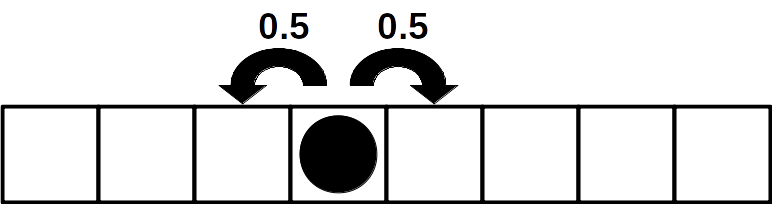
\includegraphics[width=0.8\linewidth]{gfx/1DSRW}
 \caption[\acl{srw} on a one-dimensional lattice]{\ac{srw} on a one-dimensional lattice. Black arrows indicate the possible sites in the next step with the given probabilities.}\label{fig:1DSRW}
\end{figure}

As an example, imagine the walker starting at the origin $n_0 = 0$. After one time step, its state will be $n_1=\pm 1$ with equal probability $1/2$. After another time step, accordingly, the walker can be at \mbox{$n_2=\pm 2$}, which corresponds to two consecutive steps in the same direction and has probability $1/4$, or it can be at $n_2=0$, which corresponds to two oppositely directed steps and has probability $1/2$. We can continue in this manner and decompose the number of steps $m$ into the number of steps to the right $r$ and the number of steps to the left $m-r$. Then one can argue, that the occupation probability to be at $n=2r-m$ is given by
\begin{equation*}\label{eq:srw-prob-distr}
 \P(n,m) =
 \begin{cases}
  \dbinom{m}{r}\left(\dfrac{1}{2}\right)^m & \textrm{if $n \leq m$ and $n+m$ is even}, \\
  0 & \textrm{else}.
 \end{cases}
\end{equation*}
Note that the second line follows from the condition $n+m=2r$. It is always handy to know the occupation probability, however, we do not explicitly need it in order to derive other meaningful quantities of the \ac{srw}.

Consider, for example, the \textit{mean displacement} \graffito{\textbf{Note:} We implicitly use $n_0 = 0$ and $\P(n,0)=\delta_{n,0}$ here.}
\begin{equation*}
 \avg{n_m} = \E{n_m} \equiv \sum\limits_{n=-\infty}^\infty n \P(n,m),
\end{equation*}
and the \acfi{msd}\acused{msd}
\begin{equation*}
 \avg{n_m^2} = \E{n_m^2} \equiv \sum\limits_{n=-\infty}^\infty n^2 \P(n,m).
\end{equation*}
As the single steps of the walk are independent from each other, both quantities can be easily derived as $\avg{n_m} = 0$, which illustrates the isotropy or absence of a bias, and $\avg{n_m^2} = m$, which is the typical property of diffusion (\ac{msd} linear in time). Indeed, the \ac{srw} is used to model diffusive motion \cite{codling:2008} and therefore cannot be used to model active, directed motion. However, it still serves as a good starting point for extended models.

\subsection*{Transition to continuous time and space}
Here, we want to show simple but powerful methods to derive a few properties and the occupation probability $\P(x,t)$ for the one-dimensional random walk in continuous time and space. Therefore, we first need to derive the diffusion equation, however, we only outline the derivation here. We introduce the timestep $\delta t$ and the stepsize $\delta x$. With that we can define
\begin{equation*}
 \begin{aligned}
  x &= n \cdot \delta x,
  \\
  t &= m \cdot \delta t.
 \end{aligned}
\end{equation*}
We then interpret the discrete master equation
\begin{equation*}
 \P(n, m+1) = \frac{1}{2} \P(n-1, m) + \frac{1}{2} \P(n+1, m),
\end{equation*}
accordingly to
\begin{equation*}
 \P(x, t+\delta t) = \frac{1}{2} \P(x-\delta x, t) + \frac{1}{2} \P(x+\delta x, t),
\end{equation*}
which we extend to the first non-vanishing orders of $\delta t$ and $\delta x$ and after rearranging we obtain
\begin{equation*}
 \frac{\partial \P(x, t)}{\partial t} = \dfrac{(\delta x)^2}{2 \delta t}\frac{\partial^2 \P(x, t)}{\partial x^2}.
\end{equation*}
As a last step we then take the limit $\delta x, \delta t \rightarrow 0$ in such a manner that $(\delta x)^2 / 2 \delta t = D$, where D is the diffusion coefficient, to obtain the diffusion equation
\begin{equation}\label{eq:diffusion-equation}
 \frac{\partial \P(x, t)}{\partial t} = D \frac{\partial^2 \P(x, t)}{\partial x^2}.
\end{equation}
We can then try to directly solve \autoref{eq:diffusion-equation} or we can alternatively try to understand the behavior of the walker.

Consider again the mean displacement. The transition to continuous time and space did not affect the isotropy and therefore there is still no bias. Thus we can simply write
\begin{equation*}
 \avg{x} = \int\limits_{-\infty}^\infty x \P(x, t) \diff x = 0.
\end{equation*}
without further knowledge of $\P(x, t)$. The \ac{msd}
\begin{equation*}
 \avg{x^2} = \int\limits_{-\infty}^\infty x^2 \P(x, t) \diff x
\end{equation*}
on the other hand is non-trivial. However, we can use dimensional analysis here in order to quickly derive a result. We can argue that the \ac{msd} should depend on the diffusion coefficient $D$ and the time $t$. If the abstract unit of length is $L$ and $T$ the time unit, then \autoref{eq:diffusion-equation} gives the dimensions:
\begin{equation*}
 [\avg{x^2}] = L^2, \quad [D] = \dfrac{L^2}{T}, \quad [t] = T.
\end{equation*}
The only way to form a dimensional correct relation from this is
\begin{equation*}
 \avg{x^2} \propto Dt,
\end{equation*}
which again is typical for diffusion. In order to derive the proportional factor one needs to put in a little more work. The correct equation reads
\begin{equation*}
 \avg{x^2} = 2Dt.
\end{equation*}

We can furthermore apply the powerful tool of dimensional analysis to the occupation probability $\P(x, t)$. It is $[\P(x, t)] = 1/L$ and therefore the quantity $\sqrt{Dt} \, \P(x, t)$ is dimensionless. Thus we can write
\begin{equation*}
 \sqrt{Dt} \, \P(x, t) = \P(\lambda),
\end{equation*}
where $\lambda$ needs to be a dimensionless quantity. The only dimensionless quantity that we can derive from $x$, $t$ and $D$ is the scaling variable $\lambda = x / \sqrt{Dt}$.  Hence, we can write the ansatz
\begin{equation*}
 \P(x, t) = \dfrac{1}{\sqrt{Dt}} \P\left(\dfrac{x}{\sqrt{Dt}}\right),
\end{equation*}
which is often referred to as the \textit{scaling ansatz}. We insert this in the diffusion equation \ref{eq:diffusion-equation} in order to reduce the problem to an ordinary differential equation of the form
\begin{equation*}
 2\P'' + \lambda \P' + \P = 0.
\end{equation*}
This ODE is easier to solve and we obtain as the final result \graffito{\textbf{Note:} In order to derive \autoref{eq:gauss-distr} we use both the symmetry condition $\P'(0) = 0$ and normalization.}
\begin{equation}\label{eq:gauss-distr}
 \P(x, t) = \dfrac{1}{\sqrt{4 \pi Dt}} \exp\left(-\dfrac{x^2}{4Dt}\right),
\end{equation}
a Gaussian probability distribution for the occupation probability of a one-dimensional random walk in continuous time and space. We will seize on this result in \autoref{ch:randomSearchStrategies}.


\section{Biased random walk}
\graffito{The \ac{srw} is a special case of the \acs{brw} for $p=1/2$.}For the discrete \acfi{brw}\acused{brw} we have the same situation as in the discrete \ac{srw} but we omit the isotropic property, \ie instead of symmetric hopping probabilities $p = q = 1/2$ we now allow asymmetric $p, q \in [0,1]$ such that they satisfy the condition $p + q = 1$ (see \autoref{fig:1DBRW}).

\begin{figure}[bth]
 \myfloatalign
 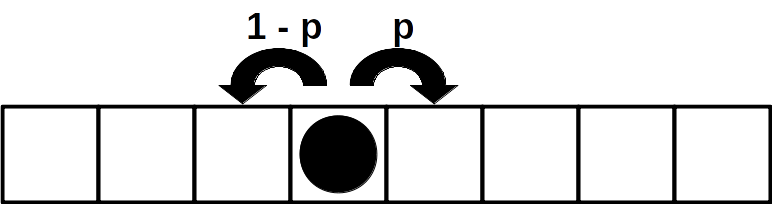
\includegraphics[width=0.8\linewidth]{gfx/1DBRW}
 \caption[\acl{brw} on a one-dimensional lattice]{\ac{brw} on a one-dimensional lattice. Black arrows indicate the possible sites in the next step with the given probabilities.}\label{fig:1DBRW}
\end{figure}

In order to compare the \ac{brw} to the \ac{srw} we again derive the mean displacement as well as the \ac{msd} as \graffito{\textbf{Note:} If we set $p=1/2$, \ie the \ac{brw} is equivalent to a \ac{srw}, we obtain the same results as for the \ac{srw}.}
\begin{equation*} 
 \begin{aligned}
  \avg{n_m} &= m (2p - 1),
  \\
  \avg{n^2_m} &= m^2 (4p^2 - 4p +1) + 4mp (1 - p).
 \end{aligned}
\end{equation*}
Thus, the walker essentially drifts to one direction, which illustrates its preference for this direction (the bias).

Furthermore, the \ac{msd} is proportional to the squared time, which is typical for \textit{ballistic motion}. However, since the mean displacement is nonzero, one can also take a look at the mean dispersal around the mean displacement, which is defined as
\begin{equation*}
 \sigma^2_m = \sum\limits_{n = -\infty}^\infty (n - \avg{n_m})^2 \P(n, m).
\end{equation*}
We obtain
\begin{equation*}
 \sigma^2_m = 4mp(1-p),
\end{equation*}
which is linear in time. In other words: in the frame which moves with the drift velocity of the walker, the motion is diffusive and not ballistic.

As we do not use the \ac{brw} in our studies, we omit the further analysis of the same. However,  we want to remark that because of its drift component, the \ac{brw} finds application in modelling search problems in which the walker has some kind of information about the direction in which it needs to move. We will consider and explain this situation in more detail later.

\section{Persistent random walk}
So far both the introduced random walk models have been uncorrelated and steps were independent from each other. In the \acfi{prw}\acused{prw} this is not the case. Instead, at a given time the hopping probabilities for the next step are dependent on the direction of the very previous step. In other words: it matters from which direction the walker came from in the previous step, \ie the walker has some kind of short memory.

In the one-dimensional discrete \ac{prw} we define a \textit{persistency} parameter $p \in [0,1]$ which represents the probability of preserving the hopping direction. Accordingly, the probability of reversing the hopping direction is $q = 1 - p$. In \autoref{fig:1DPRW} we outline the \ac{prw} again with the aid of a lattice representation, however, in opposite to the other random walks presented, here we have two possible scenarios depending on the direction of the previous step.\graffito{A \acs{prw} with persistency parameter $p=1/2$ is equivalent to the \acs{srw}.}

\begin{figure}[bth]
    \myfloatalign
    \subfloat[][]{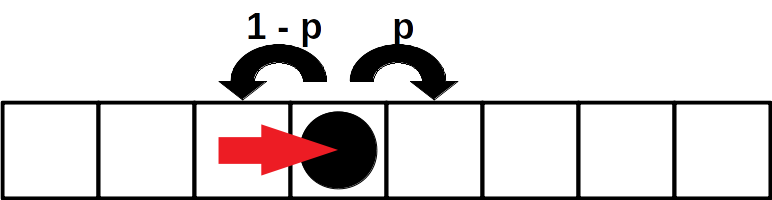
\includegraphics[width=.45\linewidth]{gfx/1DPRWfleft}} \quad
    \subfloat[][]{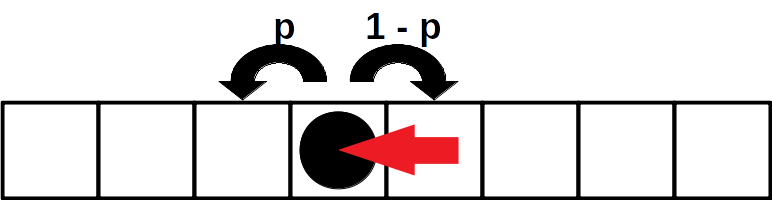
\includegraphics[width=.45\linewidth]{gfx/1DPRWfright}}
    \caption[\acl{prw} on a one-dimensional lattice]{During the one-dimensional discrete \ac{prw} the walker can step on a lattice site either by arriving from the left (a) or the right site (b). The hopping probabilities for the next step depend on the arrival direction. Red arrows indicate the arrival direction, black arrows indicate the possible sites in the next step with the given probabilities.}\label{fig:1DPRW}
\end{figure}

Consequently, walking with $p < 1/2$ tends to reverse the direction of motion in each step leading to \textit{anti-persistent motion}, while walking with $p > 1/2$ tends to preserve the direction of motion leading to \textit{persistent motion}. The trivial cases $p=0$ and $p=1$ lead to back-and-forth hopping and a straight trajectory, respectively.

Again we are interested in the mean displacement and \ac{msd}. Despite the fact that the hopping probabilities depend on the previous step, in \acp{prw}, there is no bias, \ie prefered direction of motion, in the system. Thus, the dynamics is completely different from \acp{brw}. By means of geometrical arguments or a z-Fourier-transform technique, one obtains \cite{shaebani:2014}
\begin{equation}\label{eq:reza-prw-results}
 \begin{aligned}
  \avg{n_m} &= 0,
  \\
  \avg{n^2_m} &= \frac{p}{1-p}m+\frac{2p-1}{2(1-p)^2}((2p-1)^m-1).
 \end{aligned}
\end{equation}
The mean displacement is as expected, however, the result for the \ac{msd} needs to be discussed. Therefore, we take a look at the short and long term behavior.

For short times one obtains
\begin{equation*}
 \avg{n^2_m} \propto m^\alpha,
\end{equation*}
where $\alpha = 2 + \ln{(p)} / \ln{2}$ \cite{shaebani:2014}, which leads to
\begin{equation*}
 \begin{cases}
  \alpha = -\infty \quad \hfill \textrm{(localized)} & \quad \textrm{if } p=0, \\
  -\infty < \alpha < 1 \quad \hfill \textrm{(subdiffusive)} & \quad \textrm{if } 0<p<0.5, \\
  \alpha = 1 \quad \hfill \textrm{(diffusive)} & \quad \textrm{if } p=0.5, \\
  1 < \alpha < 2 \quad \hfill \textrm{(superdiffusive)} & \quad \textrm{if } 0.5<p<1, \\
  \alpha = 2 \quad \hfill \textrm{(ballistic)} & \quad \textrm{if } p=1.
 \end{cases}
\end{equation*}
Thus, on short time scales, persistent motion, \ie $1/2 < p < 1$, is superdiffusive.

For long times, \ie $m \rightarrow \infty$, the second part of the right-hand side of \autoref{eq:reza-prw-results} becomes a constant and only the first part determines the behavior. This means that the \ac{msd} is linear in time and the motion becomes diffusive.

Therefore, the \ac{prw} in the persistent regime shows a transition from superdiffusive to diffusive motion, which classifies as a possible model to describe not only active, persistent motion but also efficient search strategies, as superdiffusive motion is usually considered an efficient way of exploring space.

We will use the \ac{prw} model throughout the next chapters in order to study different aspects of active motion. For this purpose, we briefly introduce the extensions of the model to discrete and continuous two-dimensional space.

\subsection{Persistent random walk on a two-dimensional lattice} \label{ssec:2d-lattice}
On a two-dimensional lattice, \ie $\Omega = \Z^2$, the persistency parameter $p$ again gives the probability to preserve the hopping direction. However, additionally to the probability to reverse the hopping direction, which we denote by $p_b$ here, we introduce two turning probabilities $p_l$ and $p_r$, which define the probabilities to step to the left and right, respectively, with respect to the direction of motion. \graffito{If all four directions are equally probable, \ie $p = p_b = p_l = p_r = 1/4$, the two-dimensional discrete \ac{prw} describes diffusion.}Obivously, they need to satisfy the condition $p + p_b + p_l + p_r = 1$. Analogously to the one-dimensional case we obtain four possible scenarios depending on the direction of motion, as shown in \autoref{fig:2DPRW}.

\begin{figure}[bth]
    \myfloatalign
    \subfloat[][]{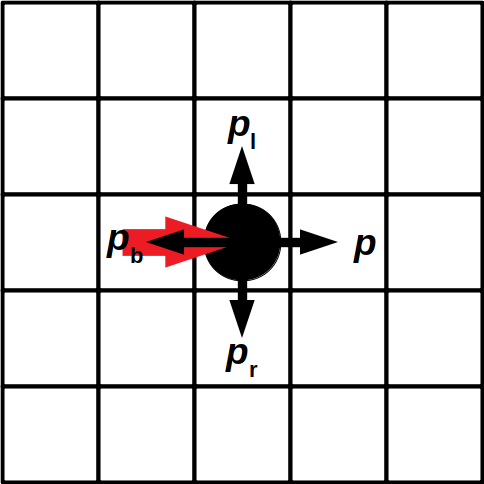
\includegraphics[width=.35\linewidth]{gfx/2DPRWfleft-small}} \quad
    \subfloat[][]{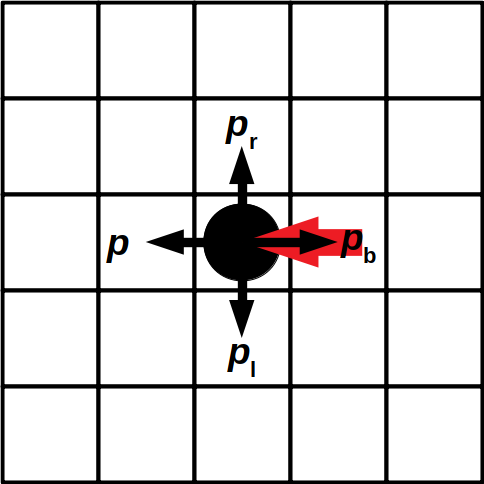
\includegraphics[width=.35\linewidth]{gfx/2DPRWfright-small}}
    \\
    \subfloat[][]{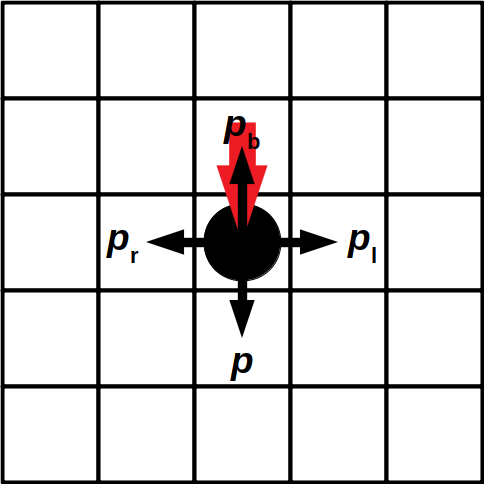
\includegraphics[width=.35\linewidth]{gfx/2DPRWftop-small}} \quad
    \subfloat[][]{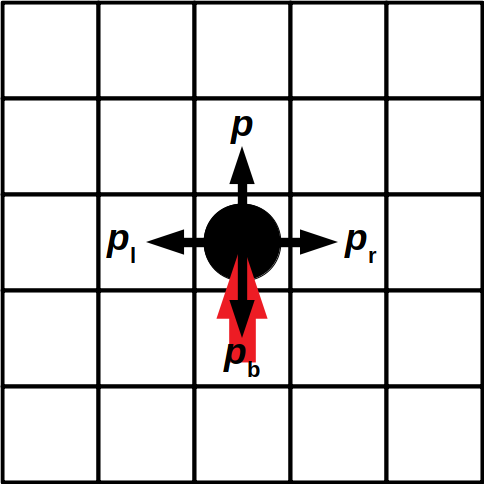
\includegraphics[width=.35\linewidth]{gfx/2DPRWfbot-small}}
    \caption[\acl{prw} on a two-dimensional lattice]{During the two-dimensional discrete \ac{prw} the walker can step on a lattice site either by arriving from the left (a), the right (b), the upper (c) or the lower site (d). The hopping probabilities for the next step depend on the arrival direction. Red arrows indicate the arrival direction, black arrows indicate the possible sites in the next step with the given probability.}\label{fig:2DPRW}
\end{figure}

Here, the analytical derivation of the mean displacement and the \ac{msd} is more lengthy than in the one-dimensional case. From the results for the one-dimensional case, however, we can assume that the mean displacement is zero and that there is a superdiffusive motion regime. For our purposes this is sufficient and we do not need to derive the explicit forms.

We return to \acp{prw} on two-dimensional lattices when the search efficiency of persistent walkers on lattices is discussed later.

\subsection{Persistent random walk in two-dimensional continuous space}
In two-dimensional continuous space, \ie $\Omega = \R^2$, instead of hopping probailities, we deal with a continuous turning angle distribution in order to determine the direction of movement. Additionally, the step-length can be chosen from a step-length distribution.

\begin{figure}[bth]
    \myfloatalign
    \subfloat[][]{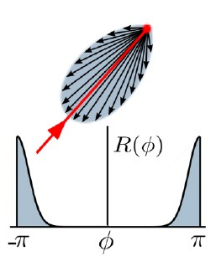
\includegraphics[width=.3\linewidth]{gfx/AntiPersTurnAngleDistri}} \quad
    \subfloat[][]{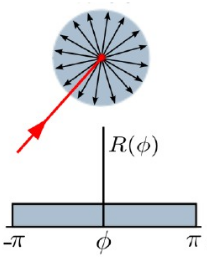
\includegraphics[width=.3\linewidth]{gfx/DiffTurnAngleDistri}} \quad
    \subfloat[][]{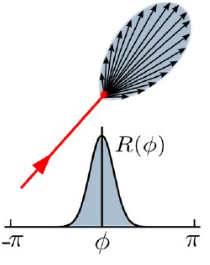
\includegraphics[width=.3\linewidth]{gfx/PersTurnAngleDistri}} 
    \caption[Turning angle distributions in the 2D \acl{prw}]{Exemplary turning angle distributions and directions of movement in the context of the two-dimensional continuous \ac{prw} for anti-persistent (a), diffusive (b) and persistent motion (c). Red arrows indicate the arrival direction, black arrows indicate possible directions in the next step, with length being proportional to the probability \cite{shaebani:2014}.}\label{fig:PRWTurningAngleDistribution}
\end{figure}

We consider the turning angle distribution $R(\phi)$ and define the mean cosine $c$ and mean sine $s$ of the turning angle as
\begin{equation*}
 \begin{aligned}
  c &= \E{\cos{\phi}} = \int\limits_{-\pi}^\pi \cos{(\phi)} R(\phi) \diff \phi,
  \\
  s &= \E{\sin{\phi}} = \int\limits_{-\pi}^\pi \sin{(\phi)} R(\phi) \diff \phi.
 \end{aligned}
\end{equation*}
These quantities hold information about the persistency of the active particle. The mean sine measures the relative probability of clockwise and anticlockwise turns. For most applications, however, the turning angle distributions are symmetric and, hence, the mean turning angle $\phi_{\textrm{mean}}$ as well as the mean sine $s$ are zero. In this case, we can use the mean cosine $c$, which measures the correlation or persistency, to define a persistency parameter $p \equiv c$. Note that, in contrast to the discrete \ac{prw}, $p\in[-1,1]$ can be negative and depending on its value, the motion is either anti-persistent (when $-1 \leq p < 0$), diffusive ($p=0$), or persistent ($0<p\leq1$). \autoref{fig:PRWTurningAngleDistribution} shows example distributions for each regime.

As a final remark, the \ac{prw} can be generalized to three dimensions as well. Although, the mathematical handling of a three-dimensional \ac{prw} can be complicated in general, if the walk is symmetric with respect to the arrival directions, the dynamics can still be described via a single persistency parameter \cite{sadjadi:2015}.

%Now that these models and methods have been briefly introduced, the two-dimensional lattice model will be slightly modified and discussed in more detail.



%*****************************************
%*****************************************
%*****************************************
%*****************************************
%*****************************************
